\documentclass[onecolumn]{ctexart}
\usepackage[utf8]{inputenc}
\usepackage{amsmath}
\usepackage{amssymb}
\usepackage{amsthm}
\usepackage{geometry}
\usepackage{graphicx}
\usepackage{float}
\usepackage{xcolor}
\usepackage{listings}
\usepackage{indentfirst}
\usepackage{bm}
\usepackage{tikz}
\usetikzlibrary{shapes,arrows}
\geometry{a4paper,scale=0.8}

\newtheorem{definition}{Definition}
\newtheorem{theorem}{Theorem}
\newtheorem{proposition}{Proposition}
\newtheorem{lemma}{Lemma}
\newtheorem{corollary}{Corollary}
\newtheorem{remark}{Remark}
\newtheorem{example}{Example}

\title{Notes of "Metric Characteristics of Conic Sections"}
\author{Jinxin Wang}
\date{}

\begin{document}

\maketitle

\section{Geometric Interpretation of Eigenvalues and Eigenvectors}

Notice that a characteristic of the major and minor axes of an ellipse is that 
the intersection between an ellipse and its major and minor axes, i.e. the vertex 
and covertex of an ellipse, have the maximum and minimum distance to the center 
respectively in the set of points on the ellipse.

In the language of analysis, let $E$ be the set of points on an ellipse 
$\varGamma$, $O$ be the center of $\varGamma$, and a function $f: E \to 
\mathbb{R}$ map a point $P \in E$ to its distance to $O$. Then the fact we stated 
above is that $f$ assumes its global maximum and minimum values on the vertex and 
covertex of $\varGamma$ respectively, and the vectors from the center $O$ to the 
vertex and covertex represent the directions of the major and minor axes of the 
ellipse $\varGamma$. Therefore, this observation might help us determine the 
symmetric axis of a quadratic curve.

Frame the problem: on the set $E$ of points $(x, y)$ such that $\frac{x^2}{a^2} 
+ \frac{y^2}{b^2} = 1$, we need to find the points on which $f(x, y) = x^2 + y^2$ 
assumes global extreme values. To reduce the difficulty, we might consider an 
easier dual problem to the original one: on the set $E$ of points $(x, y)$ such 
that $x^2 + y^2 = 1$, we need to find the points on which $f(x, y) = 
\frac{x^2}{a^2} + \frac{y^2}{b^2}$ assumes global extreme values.

The dual relationship between the two problems can be understood in the following 
way:
\begin{itemize}
  \item Ratio
  
  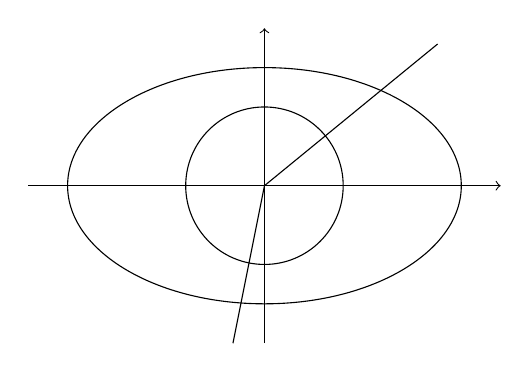
\begin{tikzpicture}
    \draw[->] (-3, 0) -- (3, 0);
    \draw[->] (0, -2) -- (0, 2);
    \draw (0, 0) ellipse (2.5 and 1.5);
    \draw (0, 0) circle (1);
    \draw (0, 0) -- (2.2, 1.8);
    \draw (0, 0) -- (-0.4, -2);
  \end{tikzpicture}
  \item Change of basis
\end{itemize}

Recall that a global extremum is also a local extramum, and a necessary condition 
for an interior extremum of a differentiable function at the point is that the 
derivative is $0$.

\begin{proposition}
  Given the equation of a quadratic curve $\varGamma$ in a plane:
  \[
    F(x, y) = (x, y, 1)A[x, y, 1] = 0
  \]
  where $A$ is the associated symmetric matrix, we define two values
  \begin{equation}
    \lambda_1 = \sup \lbrace (x,y)A_0[x,y] \mid x^2 + y^2 = 1 \rbrace
  \end{equation}
  \begin{equation}
    \lambda_2 = \inf \lbrace (x,y)A_0[x,y] \mid x^2 + y^2 = 1 \rbrace
  \end{equation}
  then we have the following conclusions:
  \begin{description}
    \item[C1] $\lambda_1$ and $\lambda_2$ are two eigenvalues of $\varGamma$.
    \item[C2] There exist unit vectors $\vec{u}_1(m_1, n_1)$ and $\vec{u}_2(m_2, 
    n_2)$ such that 
    \[
      \lambda_1 = (m_1, n_1)A_0[m_1, n_1],\thickspace \lambda_2 = (m_2, n_2)A_0[m_2, n_2] 
    \]
    and they satisfy
    \[
      A_0[m_1, n_1] = \lambda_1[m_1, n_1],\thickspace A_0[m_2, n_2] = \lambda_2[m_2, n_2]
    \]
    In other words, $\vec{u}_1$ and $\vec{u}_2$ are eigenvectors associated with 
    $\lambda_1$ and $\lambda_2$ respectively.
    \item[C3] If $\lambda_1 \neq \lambda_2$, then $\vec{u}_1 \perp \vec{u}_2$. If 
    $\lambda_1 = \lambda_2$, then any vectors are eigenvectors of $\lambda_1$ and 
    $\lambda_2$.
  \end{description}
\end{proposition}
\begin{proof}
  Hint:
  \begin{description}
    \item[Part 1] Prove the existence of $\lambda_1$ and $\lambda_2$, and the 
    unit vectors $\vec{u}_1(m_1, n_1)$ and $\vec{u}_2(m_2, n_2)$.

    Let $x = \cos\theta$ and $y = \sin\theta$ where $\theta \in \lbrack 0, 2\pi 
    \rbrack$ (the reason behind the closed interval is to apply the property of 
    a continuous function on a compact set). In this way, 
    \[
      \begin{split}
        f(x, y) &= (x, y)A_0[x, y] \\
                &= (\cos\theta, \sin\theta)A_0[\cos\theta, \sin\theta] \\
                &= a_{11}\cos^2\theta + a_{22}\sin^2\theta + 2a_{12}\cos\theta\sin\theta
      \end{split}
    \]
    which is a continous function on $\lbrack 0, 2\pi \rbrack$.
    \item[Part 2] Prove that they satisfy
    \[
      A_0[m_1, n_1] = \lambda_1[m_1, n_1],\thickspace A_0[m_2, n_2] = \lambda_2[m_2, n_2]
    \]

    Since $\lambda_1$ and $\lambda_2$ are global extreme values of $f(\theta)$, 
    then $f'(\theta_i) = 0, i=1,2$.
    \[
      \begin{split}
        f'(\theta) &= (a_{11}\cos^2\theta + a_{22}\sin^2\theta + 2a_{12}\cos\theta\sin\theta)' \\
                   &= 2(-a_{11}\cos\theta\sin\theta + a_{12}(\cos^2\theta - \sin^2\theta) + a_{22}\cos\theta\sin\theta) \\
                   &= 2((-\sin\theta, \cos\theta)A_0[\cos\theta, \sin\theta])
      \end{split}
    \]
    Hence we have
    \[
      (-\sin\theta_i, \cos\theta_i)A_0[\cos\theta_i, \sin\theta_i] = 0, \thickspace i=1,2
    \]
    i.e. $[-\sin\theta_i, \cos\theta_i] \perp A_0[\cos\theta_i, \sin\theta_i]$. 
    Meanwhile, $[-\sin\theta_i, \cos\theta_i] \perp [\cos\theta_i, \sin\theta_i]$,
    then we have
    \[
      A_0[\cos\theta_i, \sin\theta_i] = \mu [\cos\theta_i, \sin\theta_i]
    \]
    in which if we multiply both sides with $(\cos\theta_i, \sin\theta_i)$ on the 
    left side, we get
    \[
      \begin{split}
        (\cos\theta_i, \sin\theta_i)\mu[\cos\theta_i, \sin\theta_i] &= (\cos\theta_i, \sin\theta_i)A_0[\cos\theta_i, \sin\theta_i] \\
        \mu(\cos\theta_i, \sin\theta_i)[\cos\theta_i, \sin\theta_i] &= (\cos\theta_i, \sin\theta_i)A_0[\cos\theta_i, \sin\theta_i] \\
        \mu &= \lambda_i
      \end{split}
    \]
    \item[Part 3] Prove that if $\lambda_1 \neq \lambda_2$ (TODO)
  \end{description}
\end{proof}
\end{document}